\section{Конструкторская часть}

\subsection{Постановка задачи}
Решаемая задача формулируется следующим образом: необходимо создать программное обеспечение, позволяющее работать с  нечеткими экспертными системами типа Мамдани и Сугено. Обычный пользователь может выбирать конкретную систему и получать результат при конкретных входных данных. Эксперты в зависимости от своей специализации дополнительно обладают возможностью добавлять, редактировать и удалять лингвистические переменные, функции принадлежности, правила вывода некоторых экспертных систем. Администраторы могут добавлять, изменять и удалять экспертные системы, лингвистические переменные, функции принадлежности и правила, изменять права доступа пользователей и экспертов.

В общем виде задача разрабатываемого ПО представлена на рисунке \ref{fig:idef} и заключается в получении результата работы нечеткой экспертной системы с определенными параметрами на основе входных данных.

\begin{figure}[H]
	\centering
	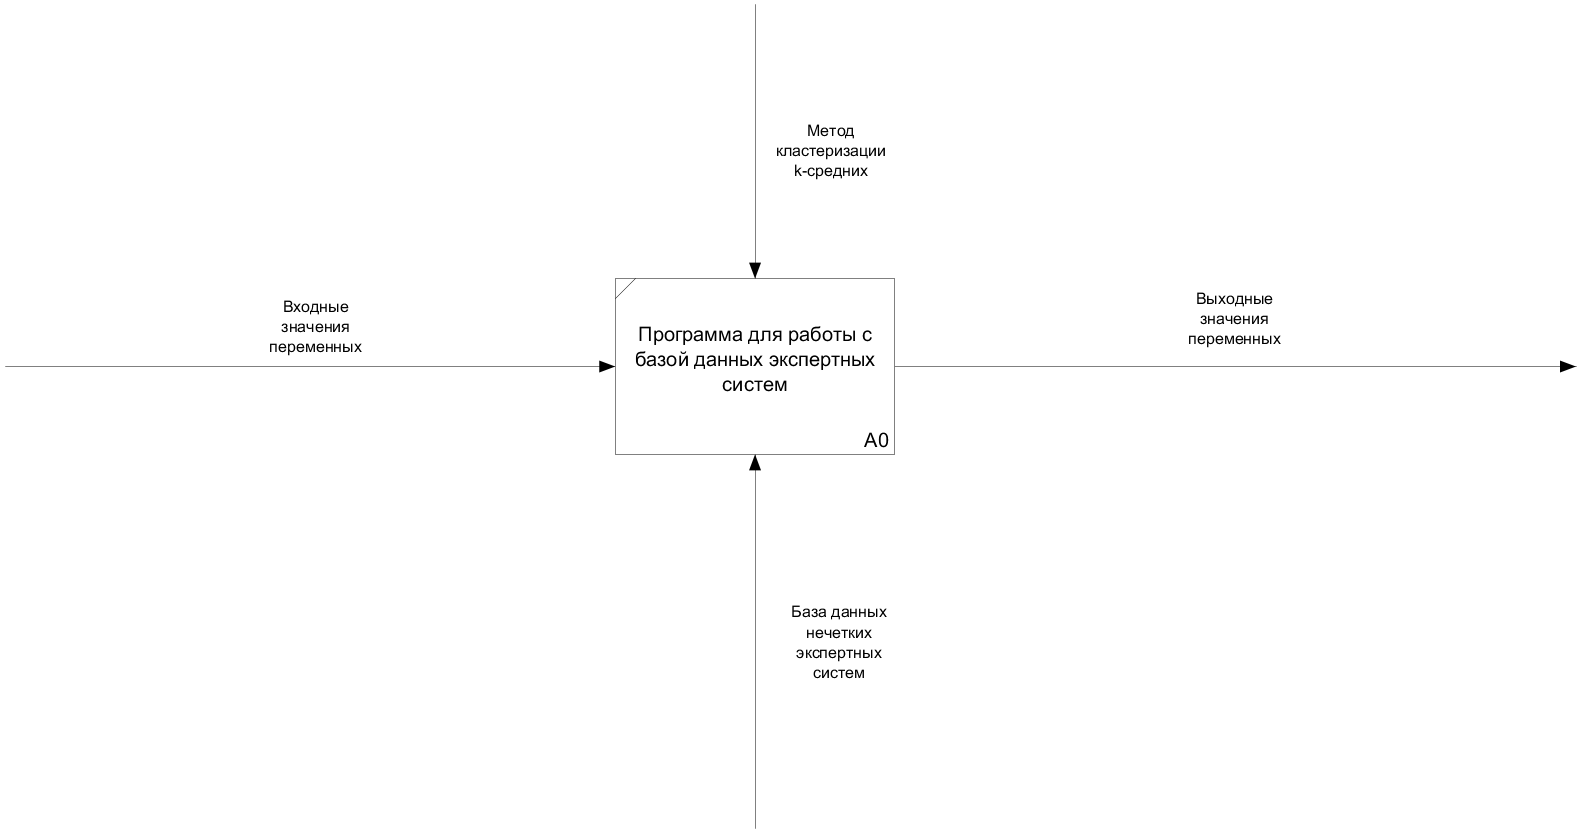
\includegraphics[width=1\linewidth]{img/Idef.png}
	\caption{Постановка задачи}
	\label{fig:idef}
\end{figure}

Диаграмма прецедентов для различных пользователей представлена на рисунке \ref{fig:use-case}.

\begin{figure}[H]
	\centering
	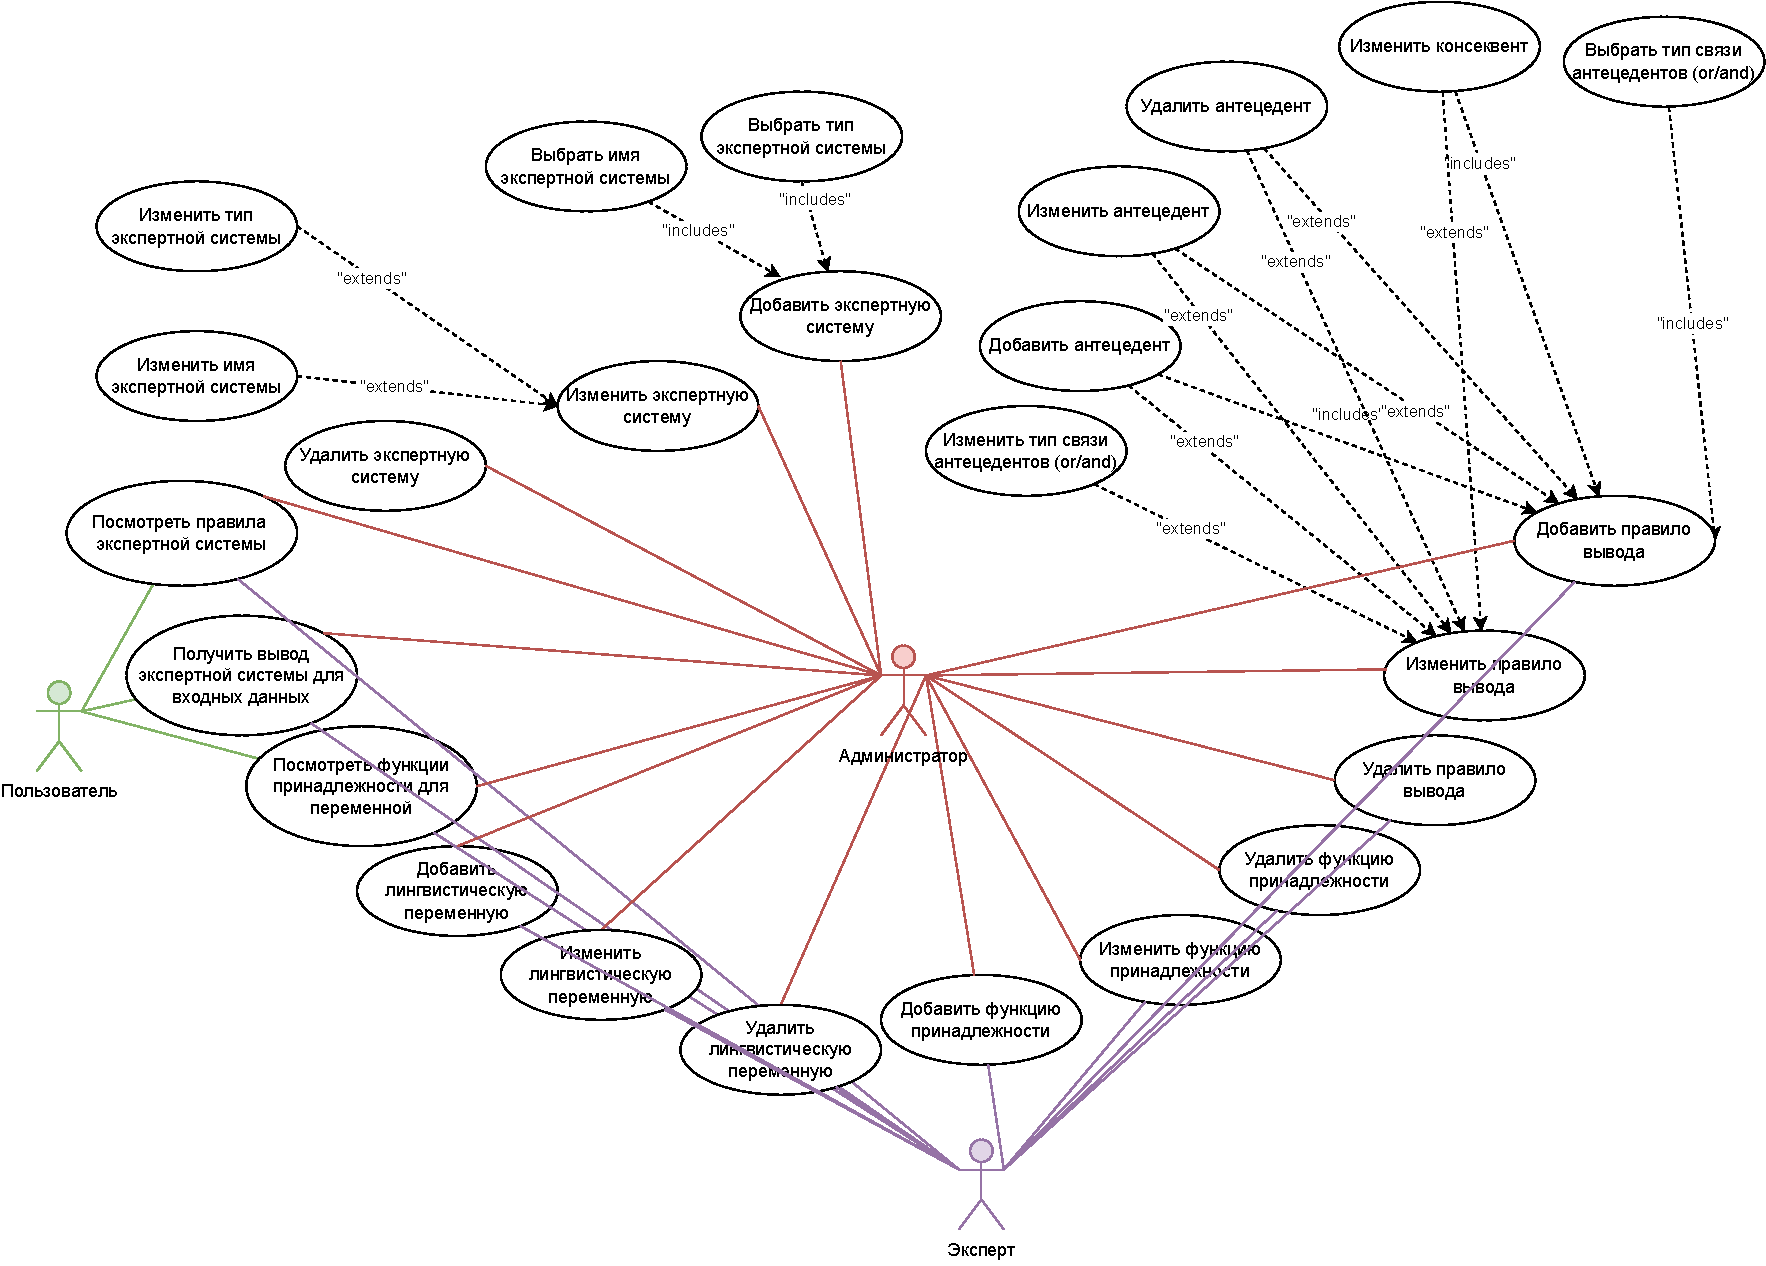
\includegraphics[width=1\linewidth]{img/use-case}
	\caption{Диаграмма вариантов использования разрабатываемого продукта}
	\label{fig:use-case}
\end{figure}

\subsection{Представление в базе данных}
Для реализации базы данных, хранящей информацию о нечетких экспертных системах, необходимо выделить сущности. Диаграмма <<сущность--связь>> разрабатываемой базы данных представлена на рисунке \ref{fig:fuzzysystemdatabasediagram}.

Таблица system отвечает за хранение следующей информации о нечеткой экспертной системе:
\begin{itemize}
	\item s\_id -- уникальный идентификатор системы в базе данных;
	\item s\_name -- название нечеткой экспертной системы;
	\item s\_type -- тип нечеткой экспертной системы (Мамдани или Сугено);
	\item specialization -- специализация нечеткой экспертной систем (физика, химия, информатика) для разделения прав доступа экспертов.
\end{itemize}

Таблица variable хранит информацию о переменных, использующихся в экспертных системах, и имеет следующие поля:
\begin{itemize}
	\item v\_id -- уникальный идентификатор переменной в базе данных;
	\item v\_name -- название переменной;
	\item min\_value -- минимальное значение, принимаемое переменной;
	\item max\_value -- максимальное значение, принимаемое переменной;
	\item v\_value -- текущее значение переменной;
	\item s\_id -- внешний ключ для таблицы System, определяет, в какой системе используется переменная.
\end{itemize}

\begin{figure}[H]
	\centering
	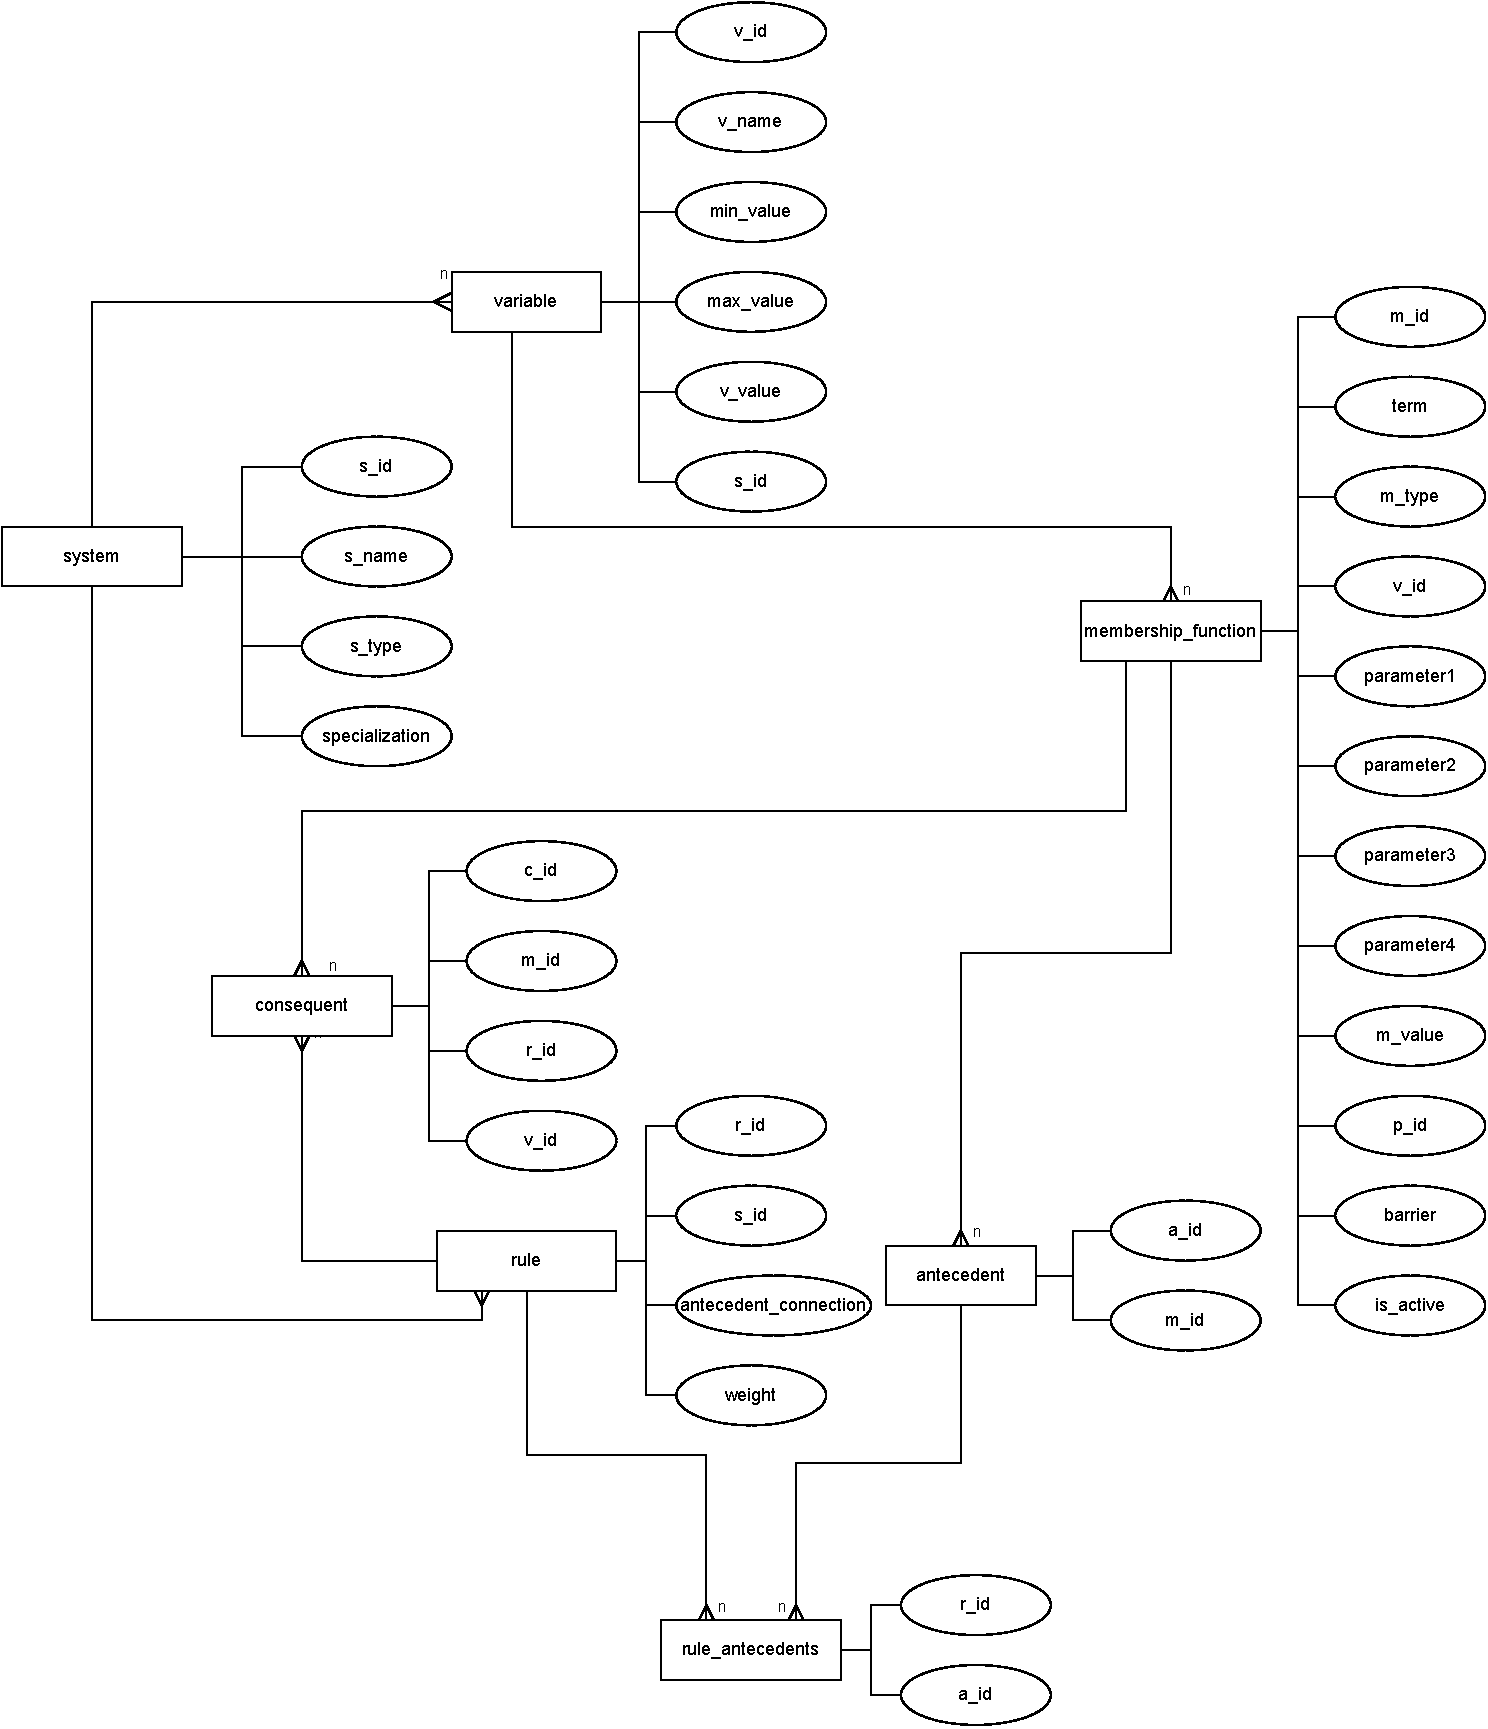
\includegraphics[width=1\linewidth]{img/FuzzySystemDatabaseDiagram}
	\caption{Диаграмма сущность-связь}
	\label{fig:fuzzysystemdatabasediagram}
\end{figure}

Таблица membership\_function хранит информацию о функциях принадлежности нечетких множеств. Структура таблицы описана ниже.
\begin{itemize}
	\item m\_id -- уникальный идентификатор функции принадлежности в базе данных;
	\item term -- лингвистический терм, связанный с функцией принадлежности;
	\item m\_type -- вид функции принадлежности: треугольная, трапециевидная, лингвистическая, S-функция, П-функция, линейная или числовая \\*(последние две используются для выражения консеквентов правил нечетких экспертных систем типа Сугено);
	\item v\_id -- связанная с функцией принадлежности переменная;
	\item parameter1, ..., parameter4 -- параметры функции принадлежности;
	\item m\_value -- текущая степень принадлежности переменной множеству;
	\item p\_id -- внешний ключ для таблицы membership\_function, используется для лингвистических функций, определяет, к какому множеству применяется лингвистический барьер;
	\item barrier -- лингвистический барьер;
	\item is\_active -- флаг, определяющий, используется ли функция для правил вывода в данный момент.
\end{itemize}

Для хранения правил вывода используются таблицы rule, consequent, \\*antecedent и rule\_antecedents. У каждого правила может быть несколько антецедентов, при этом один и тот же антецедент может входить в несколько правил.

В таблице rule хранится следующая информация о правилах вывода:
\begin{itemize}
	\item r\_id -- уникальный идентификатор правила в базе данных;
	\item s\_id -- внешний ключ для таблицы system, описывает, к какой системе относится правило вывода;
	\item antecedent\_connection -- вид соединения антецедентов (<<и>> или <<или>>);
	\item weight -- вес правила.
\end{itemize}

Таблица antecedent хранит информацию об антецедентах правил и имеет представленную ниже структуру.
\begin{itemize}
	\item a\_id -- уникальный идентификатор антецедента в системе;
	\item m\_id -- внешний ключ для таблицы membership\_function, которая задает условие <<если x есть Y>>, где x -- переменная, Y -- нечеткое множество.
\end{itemize}

Таблица rule\_antecendents связывает антецеденты с правилами и состоит только из внешних ссылок на соответствующие таблицы.

Таблица consequent описывает консеквенты правил и имеет следующие поля:
\begin{itemize}
	\item c\_id -- уникальный идентификатор консеквента в базе данных;
	\item m\_id -- связанная с консеквентом функция принадлежности (для систем типа Мамдани описывает выражение <<x есть Y>>, где x -- переменная, Y -- нечеткое множество; для систем типа Сугено -- отдельное слагаемое для линейной функции принадлежности выходной переменной);
	\item r\_id -- внешний ключ для таблицы rule, описывает, частью какого правила является консеквент;
	\item v\_id -- внешний ключ для таблицы variable, для правил типа Сугено описывает выходную переменную.
\end{itemize}

\subsection{Разработка алгоритмов}

Из-за специфики баз данных необходимо определить хранимые процедуры и триггеры для полноценной работы экспертных систем. Для этого понадобятся следующие функции:
\begin{enumerate}
	\item Вычисление значений функций принадлежности каждого из типов (треугольной, трапециевидной, s-функции, $\Pi$-функции, лингвистической) \\*при обновлении значения связанной с ними лингвистической переменной \\*(триггер).
	\item Вычисление результата работы нечеткой экспертной системы (функции):
	\begin{enumerate}
		\item типа Сугено:
		\begin{enumerate}
			\item вычисление антецедентов;
			\item вычисление результата;
		\end{enumerate}
		\item типа Мамдани:
		\begin{enumerate}
			\item вычисление степеней принадлежности выходных переменных нечетким множествам;
			\item вычисление центров нечетких множеств при некотором значении функции принадлежности;
			\item дефаззификация методом центра тяжести для дискретных множеств.
		\end{enumerate}
	\end{enumerate}
\end{enumerate}

Функции вычисления значений функций принадлежности высчитывают значение формулам \ref{eq:tr-func}--\ref{eq:notVery}. Схемы алгоритма получения результата нечеткой экспертной системы приведены на рисунках \ref{fig:algorithm} и \ref{fig:getresultfuncs}.

\begin{figure}[H]
	\centering
	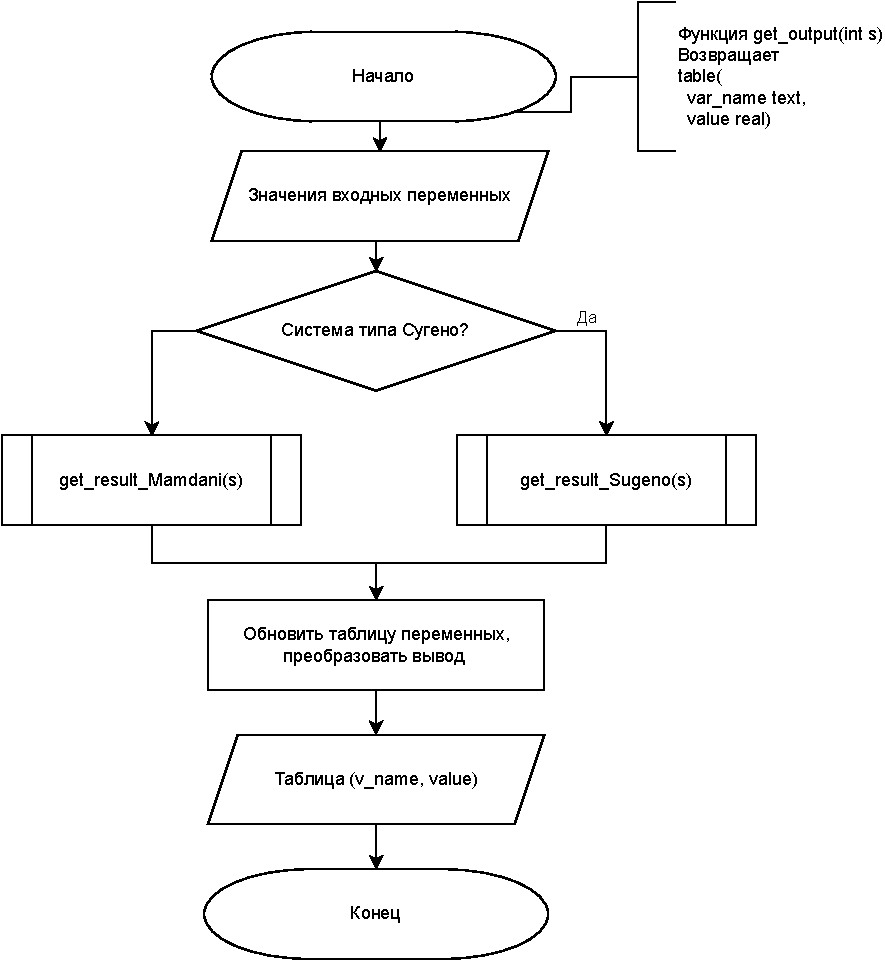
\includegraphics[width=0.7\linewidth]{img/algorithm}
	\caption{Алгоритм получения результата работы нечеткой экспертной системы в базе данных}
	\label{fig:algorithm}
\end{figure}
\begin{figure}[H]
	\centering
	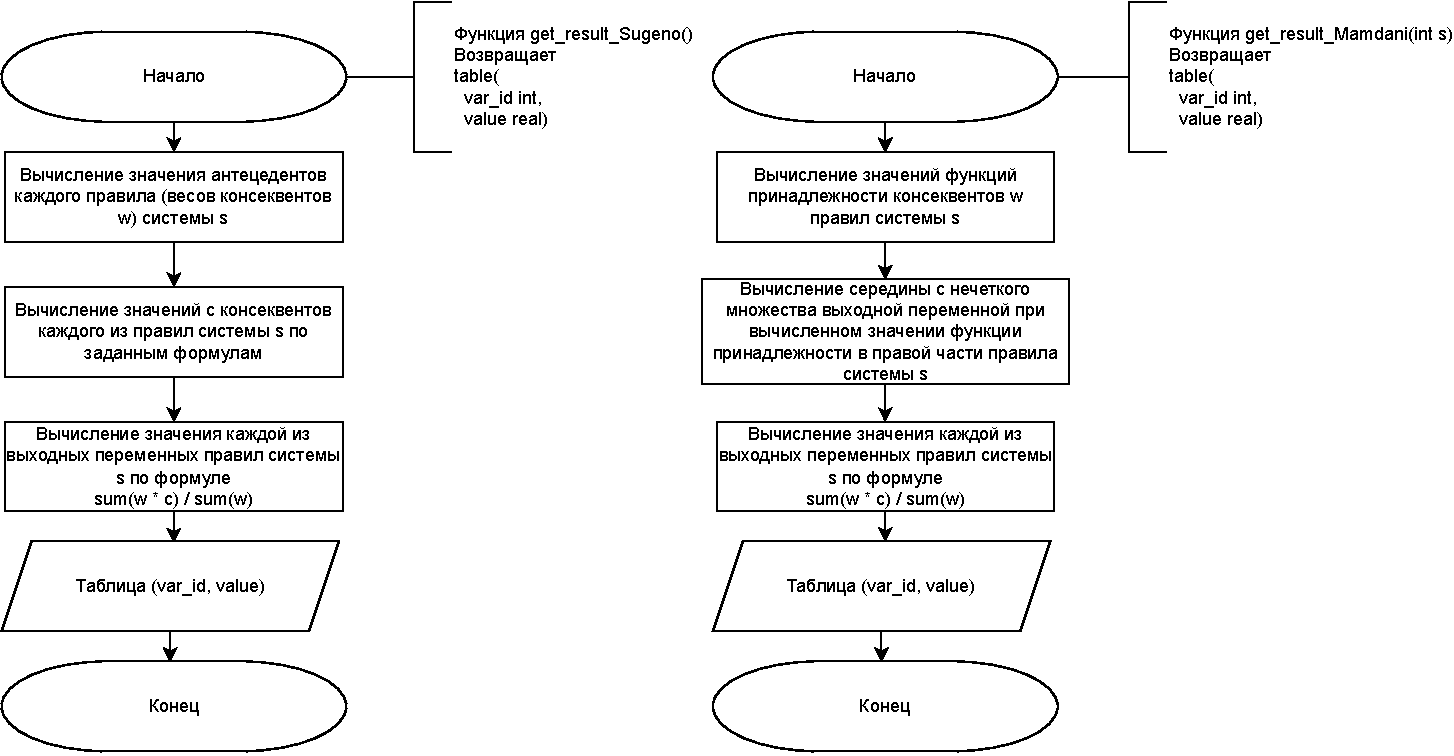
\includegraphics[width=1\linewidth]{img/get_result_funcs}
	\caption{Схема функций get\_result\_Sugeno и get\_result\_Mamdani}
	\label{fig:getresultfuncs}
\end{figure}

Реализация объектов базы данных приведена в приложении А.

\subsection{Выводы}
В данном разделе описана постановка задачи, представлены диаграммы вариантов использование и <<сущность--связь>> разрабатываемой базы данных, приведен алгоритм получения вывода нечеткой экспертной системы для баз данных.

\pagebreak